% !Mode:: "TeX:DE:UTF-8:Main"

\documentclass[aspectratio=169]{beamer}
\usepackage{tikz}
\usetikzlibrary{tikzlings}
\usepackage{bearwear}
\usetikzlibrary{decorations.text,fpu}
\usetikzlibrary {decorations.markings}

\setbeamertemplate{navigation symbols}{}

% trick taken from https://topanswers.xyz/tex?q=1989
\tikzset{
    use page relative coordinates/.style={
        shift={(current page.south west)},
        x={(current page.south east)},
        y={(current page.north west)}
    },
}

\makeatletter
\newcommand*{\slideinframe}{\number\beamer@slideinframe}
\makeatother
\ExplSyntaxOn
\let\intmod \int_mod:nn
\newcommand\calcpage
 {\int_min:nn{\int_eval:n{\int_div_truncate:nn{\slideinframe}{5}+1}}{40}}
\ExplSyntaxOff
     
\begin{document}

\def\steps{100}
\begin{frame}
  \begin{tikzpicture}[
     %use page relative coordinates,     
      remember picture,
      overlay,
      decoration={
      markings,
      mark= at position \fpeval{0.4+\slideinframe/(4*\steps)}
            with {\node{
\includegraphics[page=\calcpage,scale=0.3]{sloth}};}
            }   
    ]
    \node[anchor=north,inner sep=0pt] at (current page.north) 
     {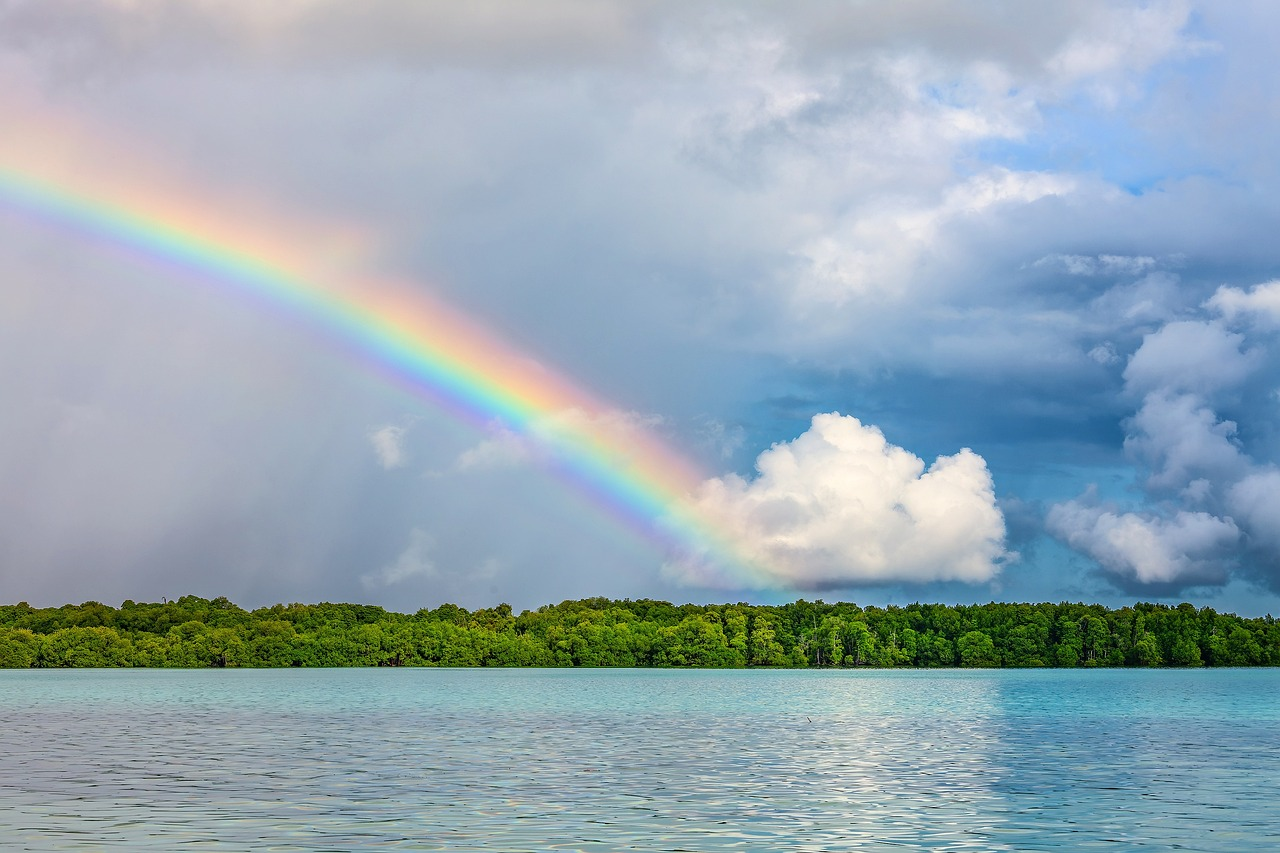
\includegraphics[width=\paperwidth]{rainbow-bg}};
      
    \node[white,text width=\paperwidth,font=\tiny,align=center] at ([yshift=0.25cm]current page.south)
       {https://pixabay.com/de/photos/landschaft-regenbogen-tropisch-7373484/};        
   
    \path[postaction=decorate]
     ([xshift=0.6\paperwidth,yshift=0.1\paperheight]current page.south west)
     to [out=110,in=180] 
     ([yshift=0.75\paperheight]current page.south west);
    
    \node at ([xshift=0.6\paperwidth,yshift=0.7\paperheight]current page.south west)
       {\includegraphics[page=\fpeval{\intmod{\slideinframe}{6}+1},scale=0.3]{bluebats}};   
    \node at ([xshift=0.5\paperwidth,yshift=0.65\paperheight]current page.south west)
         {\includegraphics[page=\fpeval{\intmod{\slideinframe+1}{6}+1},scale=0.25]{bluebats}}; 
    \node at ([xshift=0.75\paperwidth,yshift=0.55\paperheight]current page.south west)
        {\includegraphics[page=\fpeval{\intmod{\slideinframe+2}{6}+1},scale=0.35]{bluebats}}; 
  
  \end{tikzpicture} 
  
   
  \pause[\steps]
      
\end{frame}

\end{document}
